\section{Что такое дифференциальное уравнение?}
\subsection{Базовые определения}
\begin{defin}
\begin{equation}
    F\left(t,x,\frac{dx}{dt},...,\frac{d^n x}{dt^n}\right)=0 \label{ODE}
\end{equation}
- обыкновенное дифференциальное уравнение (ОДУ) порядка n.
\end{defin}
Здесь $t$ - независмая переменная,  $x(t)$ - искомая функция.
\begin{defin}
Решение ОДУ - функция $x(t)\in C^n$ (дифференцируемая n раз), обращающая
уравнение в тождество.
\end{defin}
\textbf{Примеры.} $\frac{dx}{dt}=0 $ - решение есть константа.\\
$\frac{dx}{dt}=5$. Решение $x=5t+c$.
(Так как решение зависит от параметра-константы, говорят об однопараметрическом
семействе решений. Если задать $x(0)$, то решение будет единственным, 
зависящим от начального условия).\\
$\frac{d^2 x}{dt^2}=w$ - уравнение равноускоренного 
движения. Решение: $x=\frac{wt^2}{2}+c_1t+c_2$, где  $c_1,c_2$ - начальная 
скорость и начальная координата соответственно. \\
\textbf{Пример.} Для уравнения $\frac{dx}{dt} =f(t)$, если 
функция в правой части непрерывна на отрезке $(a,b)$, тогда общее решение
имеет вид $x=\int f(t)dt$. Более точно, $t_0\in(a,b)$, тогда
$x(t)=\int\limits^t_{t_0}f(\tau)d\tau+x(0)$.
\begin{defin}
Общее решение ОДУ - множество всех решений.
\end{defin}
Естественно возникает вопрос, существует ли решение ДУ и единственно ли оно
при заданных начальных условиях? Выражается ли оно через элементарные функции?
Какова его область определения и значения?

\subsection{ДУ первого порядка, разрешенные относительно производной}
\begin{defin}
ДУ, разрешенные относительно производных - уравнения вида 
\begin{equation}
    \frac{dx}{dt}=f(t,x) \label{ODE_razresh}
\end{equation}
то есть уравнения, производная которых задана функцией в явном виде.
\end{defin}
\textbf{Пример.} $(\frac{dx}{dt})^2-x^2=0$ - не разрешенное
относительно производных, но оно раскладывается в два таких уравнения. \\
Минимальные требования к функции $f$ - определенность в области\\
Геометрический смысл уравнения \label{ODE_razresh}: 
%\begin{figure}[H]
%    \centering
%    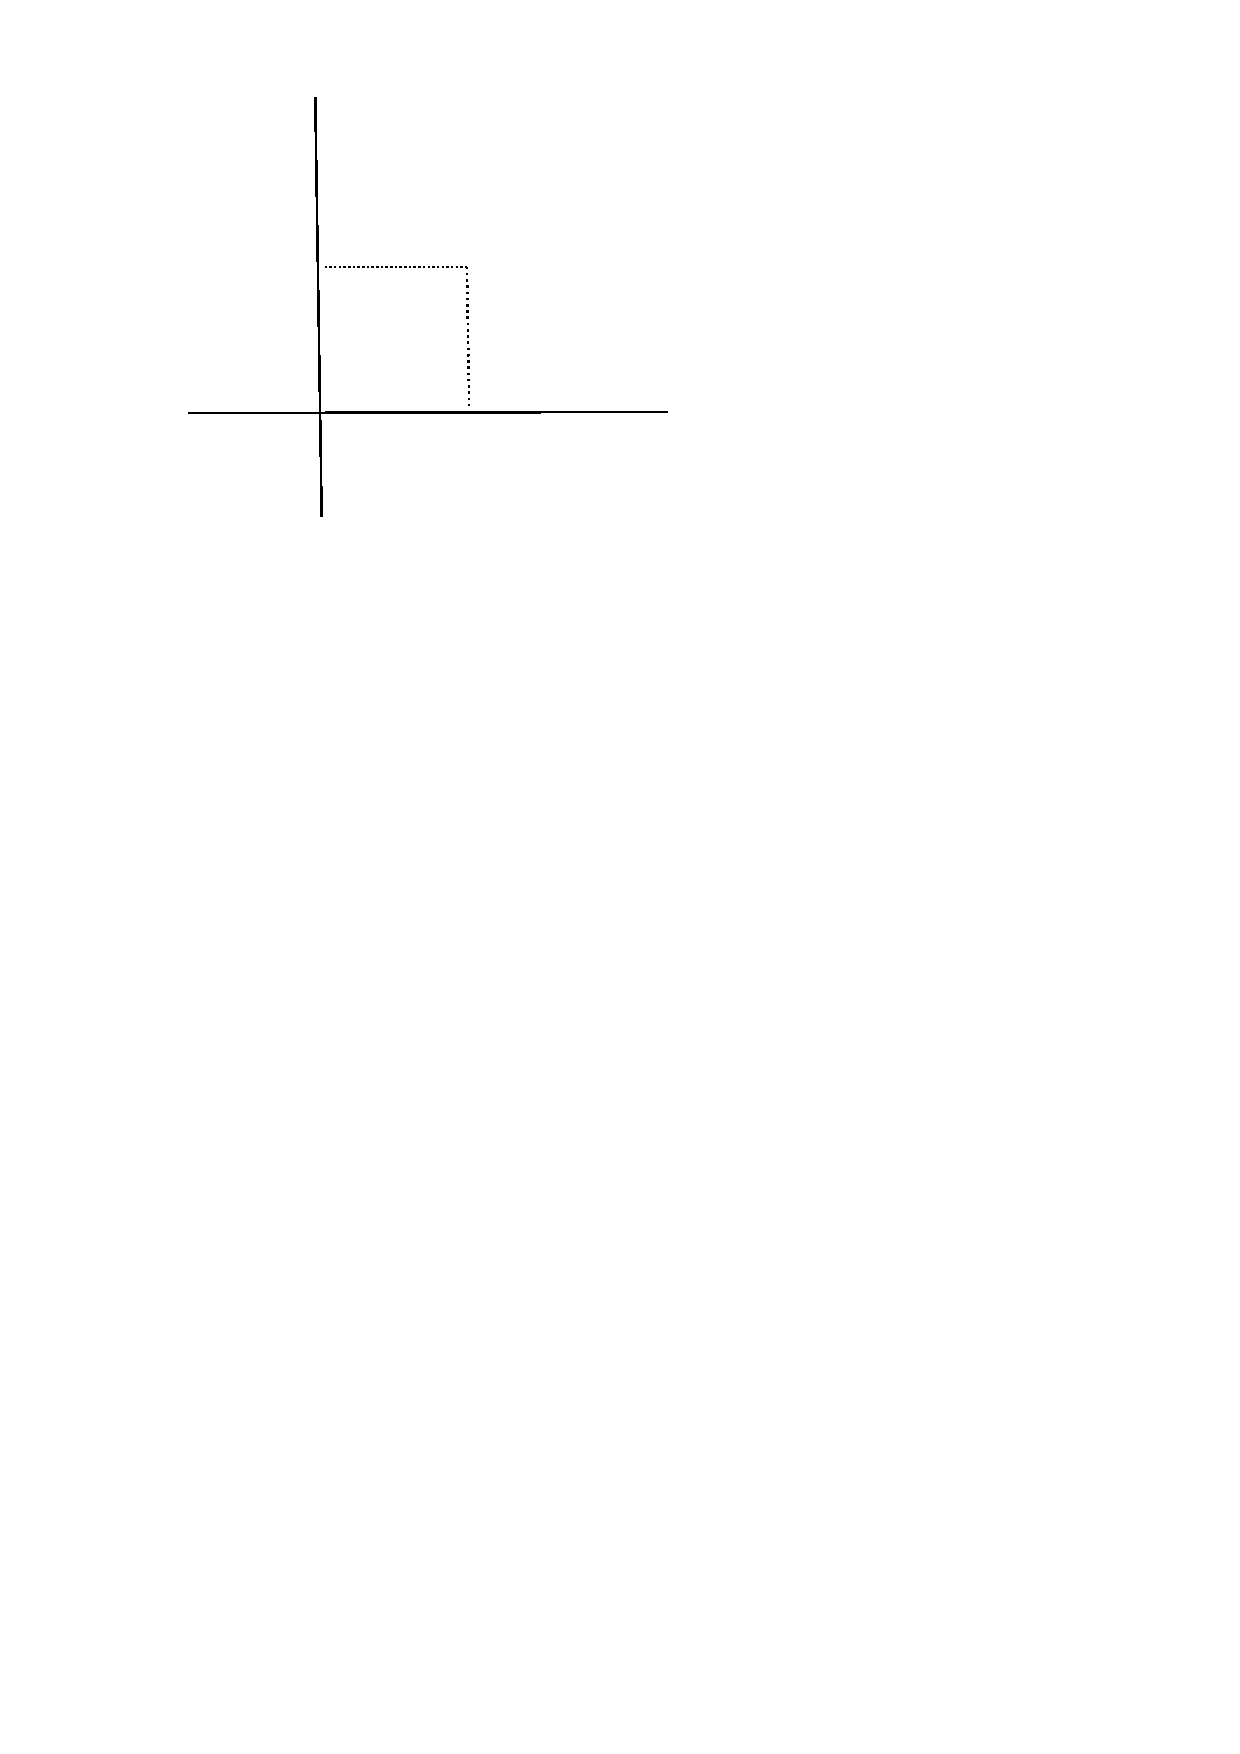
\includegraphics[width=0.8\textwidth]{figures/dir_field.pdf_tex}
%    \caption{Поле направлений на плоскости.}
%    \label{fig:dir_field}
%\end{figure}
На рисунке $\tg\tilde\alpha=f(\tilde{t},\tilde x)$\\
Говорят, что уравнение \ref{ODE_razresh} определяет поле направлений в 
\textit{расширенном} фазовом пространстве (в отличие от \textit{векторного
поля} в фазовом пространстве):
каждой точке сопоставляется направление, определяемое функцией
$f(x,t)=\tg\alpha$ (поскольку длина вектора не определена, говорят имено о 
поле направлений). Кое-кто говорит, что ДУ и поле направлений это одно и то 
же, поскольку ДУ биективно соответствуют полям направлений).\\
\textbf{Пример.} Пусть $x(t)$ - количество зараженных вирусом
в момент времени $t$. Допустим, что скорость заражения пропорциональная
количеству уже зараженных людей. Запишем это в виде ДУ:
$$\frac{dx}{dt}=kx,~k>0$$
Мы получили простейшую модель роста населения Мальтуса. Очевидно, решение
$x(t)=x_0e^{kt}$. Проблема с такой моделью состоит в том, что количество 
людей дискретно, а найденная нами функция непрерывна. Корректировка состоит
в том, что $x(t)$ понимается в смысле \textit{плотности населения}. \\
\textbf{Пример.} Рассмотрим более интересное уравнение (уравнение Бернулли,
оно же логистическое уравнение): 
$\frac{dx}{dt}=k(x)x$. Допустим, что $k(x)$ - линейная убывающая функция. 
Тогда $\frac{dx}{dt}=(k_0-\frac{k_0x}{h})x$. (Здесь $k_0=k(0),~h=k^{-1}(0)$).
Получаем нелинейное уравнение, в котором переменные не разделяются. Теперь
можно рассмотреть подробнее поле направлений. Пусть $\Gamma_0$ - множество
точек  $(t,x)$, в которых  $\frac{dx}{dt}=0$, то есть векторы поля 
параллельны оси $Ot$. Решим уравнение  $0=x(k_0-\frac{k_0}{h}x)$. \\
Получаем следующее поле: рис 2. Кривые, заключенные в середине, называются
логистическими кривыми. "Крутизна" логистической кривой зависит от параметра 
$k_0$. Данное уравнение было рассмотрено Ферхюльстом как уточнение модели
Мальтуса. 


\subsection{Метод изоклин}
Метод изоклин заключается в рисовании и исследовании графиков решений 
уравнения \ref{ODE_razresh}. 
\begin{defin}
Изоклина наклона $\alpha$ - геометрическое место точек $\Gamma_\alpha$, в 
которых касательная к решению уравнения \ref{ODE_razresh} имеет наклон, равный
$\alpha$.
\end{defin}
То есть, $\Gamma_\alpha\colon \tg\alpha=f(t,x)$\\
Опишем алгоритм метода изоклин на примере. Пусть задано уравнение 
$\frac{dx}{dt}=\frac{x}{t}$. 
\begin{enumerate}
    \item Найдем $\Gamma_0:0=\frac{x}{t}$ (то есть $x=0$ ($t\ne0$))
     Найдем $\Gamma_{90}:\frac{t}{x}=0$, то есть $t=0$ ($x\ne0$) 
    Получили, что эти гаммы есть координатные оси. 
    \item Определим области с постоянным знаком $\frac{dx}{dt}$ (среди тех,
        на которые плоскость разбивается изоклинами) 
%Почему в этих областях знак производной постоянен???
    \item Исследуем симметрии уравнений, например относительно 
    $x\to-x,~t\to-t$ (или одновременного применения). Эти симметрии
    эквивалентны отражению относительно осей.
    \item Нахождение точек перегиба и областей выпуклости, вогнутости 
интегральных кривых.  
    \item Приближенное построение интегральных кривых (то есть решений 
        уравнения).
\end{enumerate}
\textbf{Замечание.} Не все интегральные кривые являются решениями. Так, в 
рассмотренном примере ось $Ox$ - интегральная кривая, но она очевидно не 
является решением (так как не является функцией). 

Метод изоклин является качественным, и он не дает более подробной информации
о геометрии кривых. В данном конкретном примере интегральные кривые - в 
точности прямые, проходящие через точку $(0,0)$, поскольку мы заметили, что в 
каждой точке направление касательной к интегральной кривой совпадает с прямой, 
соединяющей эту точку и начало координат.\\
\textbf{Пример.} Немного изменим уравнение: $\frac{dx}{dt}=-\frac{x}{t}$. 
Главные изоклины точно такие же, как у предыдущего, а вот знаки в координатных
четвертях меняются. Поле направлений выглядит совершенно по-другому, в нем 
гиперболы. \\
\textbf{Пример.} Получим уравнение окружности с помощью ОДУ, исходя из 
следующего свойства: касательная перпендикулярна радиусу. То есть мы имеем 
некоторое поле направлений, исходя из которого можно восстановить ДУ:
$\tg\alpha=\frac{dy}{dx},~\tg\beta=\frac{y_0}{x_0}$ 
Поскольку $\alpha=\beta+90$, имеем
$\tg\alpha=\tg(\beta+90)=-\frac{1}{\tg\beta}$. В итоге уравнение имеет вид
$\frac{dy}{dx}\big|_{x=x_0}=-\frac{x_0}{y_0}$
или, если сотрем нолики (поскольку свойство универсально)
$$\frac{dy}{dx}-\frac{x}{y}$$
Заметим, что это же уравнение можно получить дифференцированием обычного
уравнения окружности. Решая его, в качестве параметра вылезет что-то, 
отвечающее за радиус. \\
Посмотрим на изоклины этого уравнения: РИС6. Ещё по приколу можно посчитать 
изоклины на $45^0$.

%Эквивалентность разных определений е
%ДЗ: №1+16(а), 16(б) $\Rightarrow$ 9









